\documentclass[border=8pt]{standalone}
\usepackage[utf8]{inputenc}
\usepackage[romanian]{babel}
\usepackage{tikz}
\usetikzlibrary{arrows.meta,decorations.pathmorphing,calc}

\begin{document}
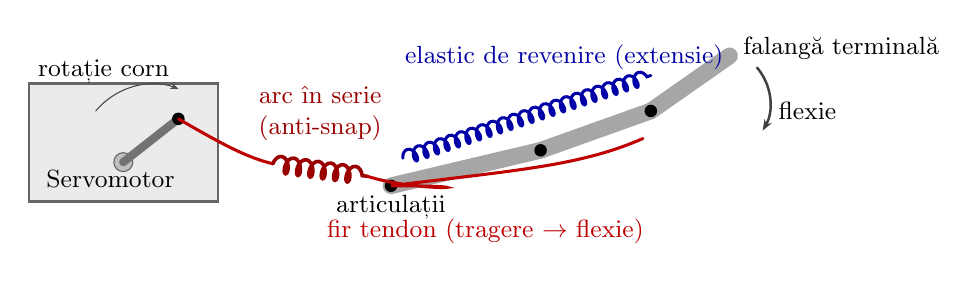
\begin{tikzpicture}[
  line cap=round,
  joint/.style={circle,fill=black,inner sep=1.6pt},
  bone/.style={line width=6pt,gray!70,line cap=round},
  tendon/.style={line width=1.1pt,red!75!black},
  elastic/.style={line width=1.1pt,blue!65!black,decorate,
                  decoration={coil,aspect=0.6,segment length=4pt,amplitude=2.5pt}},
  lab/.style={font=\small}
]

% ---- Servomotor ----
\draw[fill=black!8,draw=black!60,line width=0.8pt]
  (-0.4,-0.6) rectangle (2.0,0.9);
\node[lab,anchor=south west] at (-0.3,-0.55) {Servomotor};
% axul si cornul rotativ
\draw[fill=black!25,draw=black!60] (0.8,-0.1) circle (0.12);
\draw[line width=3pt,black!55,line cap=round] (0.8,-0.1) -- (1.5,0.45);
\node[joint] at (1.5,0.45) {};
% sageata de rotatie
\draw[-{Stealth[length=3pt]},black!70]
  (0.45,0.55) arc[start angle=140,end angle=70,radius=0.95];
\node[lab] at (0.55,1.05) {rotație corn};

% ---- Falange deget (3 segmente) ----
\coordinate (P0) at (4.2,-0.4);   % baza (MCP)
\coordinate (P1) at (6.1,0.05);   % PIP
\coordinate (P2) at (7.5,0.55);   % DIP
\coordinate (P3) at (8.5,1.25);   % varf

\draw[bone] (P0) -- (P1);
\draw[bone] (P1) -- (P2);
\draw[bone] (P2) -- (P3);
\node[joint] at (P0) {};
\node[joint] at (P1) {};
\node[joint] at (P2) {};
\node[lab,anchor=north] at (P0) {articulații};
\node[lab,anchor=west] at ($(P3)+(0.05,0.1)$) {falangă terminală};

% ---- Tendon flexor: fir -> arc puternic in serie -> fir -> deget ----
% portiune de fir (servo -> arc)
\draw[tendon] (1.5,0.45) .. controls (2.1,0.1) and (2.4,-0.05) .. (2.7,-0.12);
% arc puternic montat in serie pe fir
\draw[line width=1.3pt,red!60!black,decorate,
      decoration={coil,aspect=0.55,segment length=4.5pt,amplitude=3pt}]
  (2.7,-0.12) -- (3.9,-0.28);
% restul firului (arc -> partea palmara a degetului)
\draw[tendon] (3.9,-0.28) .. controls (4.6,-0.5) and (5.6,-0.4) ..
  (P0) .. controls (5.8,-0.2) and (6.6,-0.15) .. ($(P2)+(-0.1,-0.35)$);
\node[lab,text=red!75!black,anchor=north] at (5.4,-0.7)
  {fir tendon (tragere $\rightarrow$ flexie)};
\node[lab,text=red!60!black,anchor=south,align=center] at (3.3,0.05)
  {arc în serie\\(anti-snap)};

% ---- Elastic de revenire (partea dorsala) ----
\draw[elastic] ($(P0)+(0.15,0.35)$) -- ($(P2)+(0.0,0.45)$);
\node[lab,text=blue!65!black,anchor=south] at (6.4,0.95)
  {elastic de revenire (extensie)};

% ---- sageata directie flexie ----
\draw[-{Stealth[length=4pt]},black!75,line width=0.9pt]
  ($(P3)+(0.35,-0.15)$) arc[start angle=40,end angle=-30,radius=0.7];
\node[lab,anchor=west] at (9.0,0.55) {flexie};

\end{tikzpicture}
\end{document}
